\chapter{TikZ}

\targets{
  \item \TikZ\ kennne und lieben lernen.
  \item Pfade mit \TikZ\ zeichnen können.
  \item Das Konzept von Knoten und deren Positionierung verstehen.
  \item Kombinationsmöglichkeiten von \TikZ\ und Beamer kennen lernen.
}

\website

\section{Einführung}

\begin{Frame}{Was ist \TikZ?}
  \begin{itemize}
    \item \TikZ\ ist kein Zeichenprogramm,\\
      dient aber zum Zeichnen von Grafiken mit \LaTeX.
    \item \TikZ\ wird entwickelt und gepflegt von Till Tantau.
    \item \TikZ\ ist ein Makropaket für \TeX\ bzw. \LaTeX.
    \item \TikZ\ hat die beste Anleitung aller Zeiten.
  \end{itemize}
\end{Frame}

\begin{Frame}{Ein erstes Beispiel}
  \tikzexample{[scale=3.5]
    % Gitter im Hintergrund
    \draw[step=.5cm,gray,very thin] (0,0)
      grid (1.4,1.4);
    % Kreisbogen
    \draw (1,0) arc (0:90:1cm);
    % Koordinatenachsen
    \draw[->] (0,0) -- (1.5,0) node[right] {$x$};
    \draw[->] (0,0) -- (0,1.5) node[above] {$y$};
    % Winkel
    \filldraw[fill=green!20,draw=green!50!black]
      (0,0) -- (3mm,0pt) arc (0:30:3mm);
    \draw (15:2mm) node[green!50!black] {$\alpha$};
    % Sinus und Kosinus
    \draw[very thick,red]
      (30:1cm) -- node[left]
        {$\sin \alpha$} (30:1cm |- 0,0);
    \draw[very thick,blue]
      (30:1cm |- 0,0) -- node[below]
        {$\cos \alpha$} (0,0);
    % Schnittpunktberechnung und Tangens
    \path [name path=upward line]
      (1,0) -- (1,1);
    \path [name path=sloped line]
      (0,0) -- (30:1.5cm);
    \draw [name intersections=
      {of=upward line and sloped line, by=t}]
      [very thick,orange] (1,0) -- node [right]
      {$\displaystyle \tan \alpha \color{black}=
        \frac{{\color{red}\sin \alpha}}
          {\color{blue}\cos \alpha}$} (t);
    \draw (0,0) -- (t);
  }
\end{Frame}

\subsection{Verwendung}

\begin{Frame}[fragile]{\TikZ\ verwenden}
  \examplebox{%
    Wir arbeiten an
    \begin{tikzpicture}
      \draw (0,0) -- (1.5,0);
      \draw (0,0) -- (0,1.5);
    \end{tikzpicture}.
  }

  \xxx

  \begin{lstlisting}[gobble=4]
    \documentclass{scrartcl}
    \usepackage{tikz}
    \usetikzlibrary{intersections}
    \begin{document}
      Wir arbeiten an
      \begin{tikzpicture}
        \draw (0,0) -- (1.5,0);
        \draw (0,0) -- (0,1.5);
      \end{tikzpicture}.
    \end{document}
  \end{lstlisting}
\end{Frame}

\subsection{Pfade}

\begin{Frame}[fragile]{Pfade}
  \begin{itemize}
    \item Ein Pfad ist eine Folge von Koordinaten.
      \begin{itemize}
        \item Links unten ist \lstinline-(0,0)-,
        \item die erste Koordinate geht nach rechts und
        \item die zweite Koordinate geht nach links.
      \end{itemize}
    \item Eine Linie wird mit \lstinline|--| gezeichnet.
    \item Relative Koordinaten beginnen mit \lstinline-++-.
  \end{itemize}

  \xxx

  \tikzexample{
    \draw
      (0,0) -- ++(1,0) ++(0,1) -- ++(-1,0)
      (2,0) rectangle (3,1);
  }

  \xxx

  \begin{lstlisting}[gobble=4]
    \begin{tikzpicture}
      \draw
        (0,0) -- ++(1,0) ++(0,1) -- ++(-1,0)
        (2,0) rectangle (3,1);
    \end{tikzpicture}
  \end{lstlisting}
\end{Frame}

\begin{Frame}[t,fragile]{Gitterpfade}
  \tikzexample{
    \draw[step=0.5cm]
      (0,0) grid (1.4,1.4);
    \draw (0,0) -- (1.5,0);
    \draw (0,0) -- (0,1.5);
  }

  \xxx

  \begin{lstlisting}[gobble=4]
    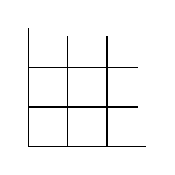
\begin{tikzpicture}
      \draw[step=0.5cm]
        (0,0) grid (1.4,1.4);
    
      \draw (0,0) -- (1.5,0);
      \draw (0,0) -- (0,1.5);
    \end{tikzpicture}
  \end{lstlisting}
\end{Frame}

\begin{Frame}[t,fragile]{Skalierung}
  \tikzexample{[scale=2]
    \draw[step=0.5cm]
      (0,0) grid (1.4,1.4);
    \draw (0,0) -- (1.5,0);
    \draw (0,0) -- (0,1.5);
  }

  \xxx

  \begin{lstlisting}[gobble=4]
    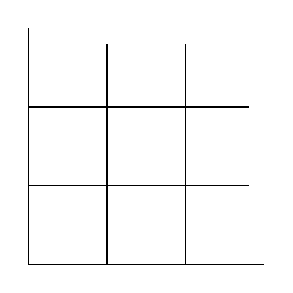
\begin{tikzpicture}[scale=2]
      \draw[step=0.5cm]
        (0,0) grid (1.4,1.4);
    
      \draw (0,0) -- (1.5,0);
      \draw (0,0) -- (0,1.5);
    \end{tikzpicture}
  \end{lstlisting}
\end{Frame}

\begin{Frame}[t,fragile]{Stile}
  \tikzexample{[scale=2]
    \draw[step=0.5cm,gray,very thin]
      (0,0) grid (1.4,1.4);
    \draw (0,0) -- (1.5,0);
    \draw (0,0) -- (0,1.5);
  }

  \xxx

  \begin{lstlisting}[gobble=4]
    \begin{tikzpicture}[scale=2]
      \draw[step=0.5cm,gray,very thin]
        (0,0) grid (1.4,1.4);
    
      \draw (0,0) -- (1.5,0);
      \draw (0,0) -- (0,1.5);
    \end{tikzpicture}
  \end{lstlisting}
\end{Frame}

\begin{Frame}[t,fragile]{Pfeilspitzen}
  \tikzexample{[scale=2]
    \draw[step=0.5cm,gray,very thin]
      (0,0) grid (1.4,1.4);
    \draw[->] (0,0) -- (1.5,0);
    \draw[->] (0,0) -- (0,1.5);
  }

  \xxx

  \begin{lstlisting}[gobble=4]
    \draw[->] (0,0) -- (1.5,0);
    \draw[->] (0,0) -- (0,1.5);
  \end{lstlisting}
\end{Frame}

\begin{Frame}[t,fragile]{Bogenpfade}
  \tikzexample{[scale=2]
    \draw[step=0.5cm,gray,very thin]
      (0,0) grid (1.4,1.4);
    \draw[->] (0,0) -- (1.5,0);
    \draw[->] (0,0) -- (0,1.5);
    %
    \draw % 0 bis 90 Grad, Radius 1 cm
      (1,0) arc (0:90:1cm)
      % 0 bis 30 Grad, Radius 3 mm
      (3mm,0pt) arc (0:30:3mm);
  }

  \xxx

  \begin{lstlisting}[gobble=4]
    \draw % 0 bis 90 Grad, Radius 1 cm
      (1,0) arc (0:90:1cm)
      % 0 bis 30 Grad, Radius 3 mm
      (3mm,0pt) arc (0:30:3mm);
  \end{lstlisting}
\end{Frame}

\begin{Frame}[t,fragile]{Farbig Zeichnen}
  \tikzexample{[scale=4]
    \clip (-.02,-.02) rectangle (1.1,0.75);
    \draw[step=0.5cm,gray,very thin]
      (0,0) grid (1.4,1.4);
    \draw[->] (0,0) -- (1.5,0);
    \draw[->] (0,0) -- (0,1.5);
    %
    \draw (1,0) arc (0:90:1cm);
    %
    \draw[green!50!black]
      (0,0) -- (3mm,0pt) arc (0:30:3mm) -- cycle;
  }

  \xxx

  \begin{lstlisting}[gobble=4]
    \draw[green!50!black]
      (0,0) -- (3mm,0pt) arc (0:30:3mm) -- cycle;
  \end{lstlisting}
\end{Frame}

\begin{Frame}[t,fragile]{Farbig Füllen}
  \tikzexample{[scale=4]
    \clip (-.02,-.02) rectangle (1.1,0.75);
    \draw[step=0.5cm,gray,very thin]
      (0,0) grid (1.4,1.4);
    \draw[->] (0,0) -- (1.5,0);
    \draw[->] (0,0) -- (0,1.5);
    %
    \draw (1,0) arc (0:90:1cm);
    %
    \fill[green!20]
      (0,0) -- (3mm,0pt) arc (0:30:3mm) -- cycle;
  }

  \xxx

  \begin{lstlisting}[gobble=4]
    \fill[green!20]
      (0,0) -- (3mm,0pt) arc (0:30:3mm) -- cycle;
  \end{lstlisting}
\end{Frame}

\begin{Frame}[t,fragile]{Farbig Zeichnen und Füllen}
  \tikzexample{[scale=4]
    \clip (-.02,-.02) rectangle (1.1,0.75);
    \draw[step=0.5cm,gray,very thin]
      (0,0) grid (1.4,1.4);
    \draw[->] (0,0) -- (1.5,0);
    \draw[->] (0,0) -- (0,1.5);
    %
    \draw (1,0) arc (0:90:1cm);
    %
    \filldraw[fill=green!20,draw=green!50!black]
      (0,0) -- (3mm,0pt) arc (0:30:3mm) -- cycle;
  }

  \xxx

  \begin{lstlisting}[gobble=4]
    \filldraw[fill=green!20,draw=green!50!black]
      (0,0) -- (3mm,0pt) arc (0:30:3mm) -- cycle;
  \end{lstlisting}
\end{Frame}

\begin{Frame}[t,fragile]{Polarkoordinaten und Schnittpunkte}
  \tikzexample{[scale=4]
    \clip (-.02,-.02) rectangle (1.1,0.75);
    \draw[step=0.5cm,gray,very thin]
      (0,0) grid (1.4,1.4);
    \draw[->] (0,0) -- (1.5,0);
    \draw[->] (0,0) -- (0,1.5);
    %
    \draw (1,0) arc (0:90:1cm);
    %
    \filldraw[fill=green!20,draw=green!50!black]
      (0,0) -- (3mm,0pt) arc (0:30:3mm) -- cycle;
    \draw[very thick,red]
      (30:1cm) -- (30:1cm |- 0,0);
    \draw[very thick,blue]
      (30:1cm |- 0,0) -- (0,0);
  }

  \xxx

  \begin{lstlisting}[gobble=4]
    \draw[very thick,red]
      (30:1cm) -- (30:1cm |- 0,0);
    \draw[very thick,blue]
      (30:1cm |- 0,0) -- (0,0);
  \end{lstlisting}
\end{Frame}

\mode
<article>

\lstinline-(30:1cm)- ist dabei die Polarkoordinate, die
den Punkt bezeichnet, der sich im Abstand von einem Zentimeter
vom Ursprung in einem Winkel von 30 Grad befindet. Das ist der
obere Punkt der roten Linie. Der untere Punkt der roten Linie
ist gleichzeitig der rechte Punkt der blauen Linie und
ergibt sich aus dem Schnittpunkt der X-Koordinate
von \lstinline-(30:1cm)- und der Y-Koordinate von
\lstinline-(0,0)-.

\mode
<all>

\begin{Frame}[t,fragile]{Schnittpunkte von Pfaden definieren}
  \tikzexample{[scale=4]
    \clip (-.02,-.02) rectangle (1.1,0.75);
    \draw[step=0.5cm,gray,very thin]
      (0,0) grid (1.4,1.4);
    \draw[->] (0,0) -- (1.5,0);
    \draw[->] (0,0) -- (0,1.5);
    %
    \draw (1,0) arc (0:90:1cm);
    %
    \filldraw[fill=green!20,draw=green!50!black]
      (0,0) -- (3mm,0pt) arc (0:30:3mm) -- cycle;
    \draw[very thick,red]
      (30:1cm) -- (30:1cm |- 0,0);
    \draw[very thick,blue]
      (30:1cm |- 0,0) -- (0,0);
    %
    \draw[name path=upward line]
      (1,0) -- (1,1);
    \draw[name path=sloped line]
      (0,0) -- (30:1.5cm);
    \draw[name intersections=
      {of=upward line and sloped line, by=t}];
  }

  \xxx

  \begin{lstlisting}[gobble=4]
    \draw[name path=upward line]
      (1,0) -- (1,1);
    \draw[name path=sloped line]
      (0,0) -- (30:1.5cm);
    \draw[name intersections=
      {of=upward line and sloped line, by=t}];
  \end{lstlisting}
\end{Frame}

\begin{Frame}[t,fragile]{Unsichtbare Pfade}
  \tikzexample{[scale=4]
    \clip (-.02,-.02) rectangle (1.1,0.75);
    \draw[step=0.5cm,gray,very thin]
      (0,0) grid (1.4,1.4);
    \draw[->] (0,0) -- (1.5,0);
    \draw[->] (0,0) -- (0,1.5);
    %
    \draw (1,0) arc (0:90:1cm);
    %
    \filldraw[fill=green!20,draw=green!50!black]
      (0,0) -- (3mm,0pt) arc (0:30:3mm) -- cycle;
    \draw[very thick,red]
      (30:1cm) -- (30:1cm |- 0,0);
    \draw[very thick,blue]
      (30:1cm |- 0,0) -- (0,0);
    %
    \path[name path=upward line]
      (1,0) -- (1,1);
    \path[name path=sloped line]
      (0,0) -- (30:1.5cm);
    \path[name intersections=
      {of=upward line and sloped line, by=t}];
  }

  \xxx

  \begin{lstlisting}[gobble=4]
    \path[name path=upward line]
      (1,0) -- (1,1);
    \path[name path=sloped line]
      (0,0) -- (30:1.5cm);
    \path[name intersections=
      {of=upward line and sloped line, by=t}];
  \end{lstlisting}
\end{Frame}

\begin{Frame}[t,fragile]{Schnittpunkte von Pfaden verwenden}
  \tikzexample{[scale=4]
    \clip (-.02,-.02) rectangle (1.1,0.75);
    \draw[step=0.5cm,gray,very thin]
      (0,0) grid (1.4,1.4);
    \draw[->] (0,0) -- (1.5,0);
    \draw[->] (0,0) -- (0,1.5);
    %
    \draw (1,0) arc (0:90:1cm);
    %
    \filldraw[fill=green!20,draw=green!50!black]
      (0,0) -- (3mm,0pt) arc (0:30:3mm) -- cycle;
    \draw[very thick,red]
      (30:1cm) -- (30:1cm |- 0,0);
    \draw[very thick,blue]
      (30:1cm |- 0,0) -- (0,0);
    %
    \path[name path=upward line]
      (1,0) -- (1,1);
    \path[name path=sloped line]
      (0,0) -- (30:1.5cm);
    \path[name intersections=
      {of=upward line and sloped line, by=t}];
    \draw[very thick,orange]
      (1,0) -- (t);
    \draw
      (0,0) -- (t);
  }

  \xxx

  \begin{lstlisting}[gobble=4]
    \draw[very thick,orange]
      (1,0) -- (t);
    \draw
      (0,0) -- (t);
  \end{lstlisting}
\end{Frame}

\subsection{Knoten}

\begin{Frame}[t,fragile]{Beschriftungen}
  \tikzexample{[scale=4]
    \clip (-.02,-.1) rectangle (1.1,0.75);
    \draw[step=0.5cm,gray,very thin]
      (0,0) grid (1.4,1.4);
    \draw[->] (0,0) -- (1.5,0);
    \draw[->] (0,0) -- (0,1.5);
    %
    \draw (1,0) arc (0:90:1cm);
    %
    \filldraw[fill=green!20,draw=green!50!black]
      (0,0) -- (3mm,0pt) arc (0:30:3mm) -- cycle;
    \draw[very thick,red]
      (30:1cm) -- node[left] {$\sin \alpha$} (30:1cm |- 0,0);
    \draw[very thick,blue]
      (30:1cm |- 0,0) -- node[below] {$\cos \alpha$} (0,0);
    %
    \path[name path=upward line]
      (1,0) -- (1,1);
    \path[name path=sloped line]
      (0,0) -- (30:1.5cm);
    \path[name intersections=
      {of=upward line and sloped line, by=t}];
    \draw[very thick,orange]
      (1,0) -- (t);
    \draw
      (0,0) -- (t);
  }

  \xxx

  \begin{lstlisting}[gobble=4]
    \draw[very thick,red]
      (30:1cm) -- node[left]
        {$\sin \alpha$} (30:1cm |- 0,0);
    \draw[very thick,blue]
      (30:1cm |- 0,0) -- node[below]
        {$\cos \alpha$} (0,0);
  \end{lstlisting}
\end{Frame}

\begin{Frame}[t,fragile]{Beschriftungen der Achsen}
  \tikzexample{[scale=2]
    \draw[step=0.5cm,gray,very thin]
      (0,0) grid (1.4,1.4);
    \draw[->] (0,0) -- (1.5,0) node[right] {$x$};
    \draw[->] (0,0) -- (0,1.5) node[above] {$y$};
    %
    \draw (1,0) arc (0:90:1cm);
    %
    \filldraw[fill=green!20,draw=green!50!black]
      (0,0) -- (3mm,0pt) arc (0:30:3mm) -- cycle;
    \draw[very thick,red]
      (30:1cm) -- node[left] {$\sin \alpha$} (30:1cm |- 0,0);
    \draw[very thick,blue]
      (30:1cm |- 0,0) -- node[below] {$\cos \alpha$} (0,0);
    %
    \path[name path=upward line]
      (1,0) -- (1,1);
    \path[name path=sloped line]
      (0,0) -- (30:1.5cm);
    \path[name intersections=
      {of=upward line and sloped line, by=t}];
    \draw [name intersections={of=upward line and sloped line, by=t}]
      [very thick,orange] (1,0) -- (t);
    \draw
      (0,0) -- (t);
  }

  \xxx

  \begin{lstlisting}[gobble=4]
    \draw[->] (0,0) -- (1.5,0) node[right] {$x$};
    \draw[->] (0,0) -- (0,1.5) node[above] {$y$};
  \end{lstlisting}
\end{Frame}

\begin{Frame}[fragile]{Vollständiges Beispiel}
  \tikzexample{[scale=3.5]
    % Gitter im Hintergrund
    \draw[step=.5cm,gray,very thin] (0,0)
      grid (1.4,1.4);
    % Kreisbogen
    \draw (1,0) arc (0:90:1cm);
    % Koordinatenachsen
    \draw[->] (0,0) -- (1.5,0) node[right] {$x$};
    \draw[->] (0,0) -- (0,1.5) node[above] {$y$};
    % Winkel
    \filldraw[fill=green!20,draw=green!50!black]
      (0,0) -- (3mm,0pt) arc (0:30:3mm);
    \draw (15:2mm) node[green!50!black] {$\alpha$};
    % Sinus und Kosinus
    \draw[very thick,red]
      (30:1cm) -- node[left]
        {$\sin \alpha$} (30:1cm |- 0,0);
    \draw[very thick,blue]
      (30:1cm |- 0,0) -- node[below]
        {$\cos \alpha$} (0,0);
    % Schnittpunktberechnung und Tangens
    \path [name path=upward line]
      (1,0) -- (1,1);
    \path [name path=sloped line]
      (0,0) -- (30:1.5cm);
    \draw [name intersections=
      {of=upward line and sloped line, by=t}]
      [very thick,orange] (1,0) -- node [right]
      {$\displaystyle \tan \alpha \color{black}=
        \frac{{\color{red}\sin \alpha}}
          {\color{blue}\cos \alpha}$} (t);
    \draw (0,0) -- (t);
  }
\end{Frame}

\begin{Frame}[fragile,allowframebreaks]{Quelltext des vollständiges Beispiel}
  \begin{lstlisting}[gobble=4]
    % Gitter im Hintergrund
    \draw[step=.5cm,gray,very thin] (0,0)
      grid (1.4,1.4);
    % Kreisbogen
    \draw (1,0) arc (0:90:1cm);
    % Koordinatenachsen
    \draw[->] (0,0) -- (1.5,0) node[right] {$x$};
    \draw[->] (0,0) -- (0,1.5) node[above] {$y$};
    % Winkel
    \filldraw[fill=green!20,draw=green!50!black]
      (0,0) -- (3mm,0pt) arc (0:30:3mm);
    \draw (15:2mm) node[green!50!black] {$\alpha$};
    % Sinus und Kosinus
    \draw[very thick,red]
      (30:1cm) -- node[left]
        {$\sin \alpha$} (30:1cm |- 0,0);
    \draw[very thick,blue]
      (30:1cm |- 0,0) -- node[below]
        {$\cos \alpha$} (0,0);
    % Schnittpunktberechnung und Tangens
    \path [name path=upward line]
      (1,0) -- (1,1);
    \path [name path=sloped line]
      (0,0) -- (30:1.5cm);
    \draw [name intersections=
      {of=upward line and sloped line, by=t}]
      [very thick,orange] (1,0) -- node [right]
      {$\displaystyle \tan \alpha \color{black}=
        \frac{{\color{red}\sin \alpha}}
          {\color{blue}\cos \alpha}$} (t);
    \draw (0,0) -- (t);
  \end{lstlisting}
\end{Frame}

\section{Graphen}

\subsection{Knoten}

\begin{Frame}{Wofür Knoten?}
  \begin{itemize}
    \item \alert{Wir können jetzt alles zeichnen.}
    \item Viele Zeichnungen basieren auf Graphen,\\
      bestehen also aus Knoten und Kanten.
      \begin{itemize}
        \item Turing-Maschinen, Automaten, Petri-Netze, \dots
        \item UML-Diagramme, Programmablaufpläne, Entity-Relationship-Diagramme, \dots
        \item Stoffwechselwege, Geschäftsprozessdiagramme, Organigramme, \dots
        \item formlose Diagramme für Beziehungen oder Abläufe,
        \item \dots
      \end{itemize}
    \item Solche Diagramme mit Kreisen und Linien zu zeichnen erzeugt
      \alert{unübersichtlichen und schlecht wartbaren} \LaTeX-Code.
  \end{itemize}
\end{Frame}

\begin{Frame}{Ein zweites Beispiel}
  \tikzexample{
    [io/.style={trapezium, trapezium left angle=70, trapezium right angle=110, fill=magenta!10, draw=magenta},
    operation/.style={rectangle, fill=orange!10, draw=orange},
    decision/.style={diamond, aspect=2, inner sep=2pt, fill=red!10, draw=red},
    node distance=5mm, thick]
    \node[io] (input) {Eingabe $a,b$};
    \node[operation, below=of input] (div) {$r=a \mod b$};
    \node[operation, below=of div] (set) {$a=b,\ b=r$};
    \node[decision, below=of set] (decision) {$b=0?$};
    \node[io, below=of decision] (output) {Ausgabe $a$};
    %
    \draw
      (input) edge[->] (div)
      (div) edge[->] (set)
      (set) edge[->] (decision)
      (decision) edge[->] node[right] {Ja} (output);
    \draw[->] (decision) -- node[below] {Nein} ++(1.5,0) |- (div);
  }
\end{Frame}

\begin{Frame}[fragile]{Todo}
  \begin{verbatim}
    \path (0,0) node {Foo};
    at-Syntax
    Stile und inner sep
    Knoten benennen
    Relative Positionierung
    Kanten
    Kanten beschriften
  \end{verbatim}
\end{Frame}

\subsection{Automaten}

\begin{Frame}[fragile]{Automaten}
  \tikzexample{[auto, thick]
    \node[initial,state] (q0) {$q_0$};
    \visible<2->{\node[state, right=of q0] (q1) {$q_1$};}
    \visible<3->{\node[state, accepting, right=of q1] (q2) {$q_2$};}
    \visible<2->{\draw
      (q0) edge[->] node {0} (q1)
      (q1) edge[->, loop above] node {0} ();}
    \visible<3->{\draw
      (q1) edge[->, bend left] node {1} (q2)
      (q2) edge[->, bend left] node {0} (q1);}
  }

  \xxx

  \begin{lstlisting}[gobble=4,escapechar=\%]
    \tikz[auto, thick]{
      %\pause[1]%\node[initial, state] (q0) {$q_0$};            %\onslide%
      %\pause[2]%\node[state, right=of q0] (q1) {$q_1$};        %\onslide%
      %\pause[3]%\node[state, accepting, right=of q1]           %\onslide%
      %\pause[3]%  (q2) {$q_2$};                                %\onslide%
      %\pause[2]%\draw (q0) edge[->] node {0} (q1)              %\onslide%
      %\pause[2]%      (q1) edge[->, loop above] node {0} ()    %\onslide%
      %\pause[3]%           edge[->, bend left] node {1} (q2)   %\onslide%
      %\pause[3]%      (q2) edge[->, bend left] node {0} (q1)%\pause[2]%;%\onslide%}
  \end{lstlisting}
\end{Frame}

\subsection{Bäume}

\begin{Frame}[fragile]{Bäume}
  \begin{columns}
    \column{42mm}
      \tikzexample{[
        every node/.style={draw,circle,inner sep=0pt,minimum width=15pt},%
        edge from parent/.style={},%
        level/.style={sibling distance=20mm/#1},%
        level distance=10mm, thick]
        \node[coordinate] (root) {}
          child { child child }
          child { child child };
        %  
        \node at (root) (a) {a};
        \visible<2->{\node at (root-1) (b) {b};}
        \visible<4->{\node at (root-2) (e) {e};}
        \visible<3->{\node at (root-1-1) (c) {c};}
        \visible<3->{\node at (root-1-2) (d) {d};}
        \visible<5->{\node at (root-2-1) (f) {f};}
        \visible<5->{\node at (root-2-2) (g) {g};}
        \visible<2->{\path (a) edge (b);}
        \visible<4->{\path (a) edge (e);}
        \visible<3->{\path (b) edge (c)
                       edge (d);}
        \visible<5->{\path (e) edge (f)
                       edge (g);}
      }
    
    \column{52mm}
    
    \begin{lstlisting}[gobble=6,escapechar=\%]
      %\pause[1]%\node {a}                %\onslide%
      %\pause[2]%  child { node {b}       %\onslide%
      %\pause[3]%    child { node {c} }   %\onslide%
      %\pause[3]%    child { node {d} }   %\onslide%
      %\pause[2]%  }                      %\onslide%
      %\pause[4]%  child { node {e}       %\onslide%
      %\pause[5]%    child { node {f} }   %\onslide%
      %\pause[5]%    child { node {g} }   %\onslide%
      %\pause[4]%  }%\onslide%;
    \end{lstlisting}
  \end{columns}
\end{Frame}

\begin{Frame}[fragile]{Ganzer \LaTeX-Code des Baums}
  \begin{lstlisting}[gobble=4]
    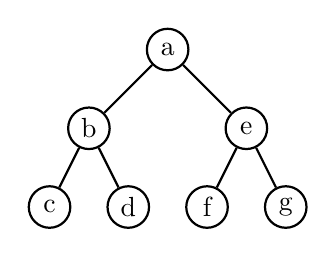
\begin{tikzpicture}[
      every node/.style={draw,circle,inner sep=0pt,
        minimum width=15pt},
      level/.style={sibling distance=20mm/#1},
      level distance=10mm, thick]
      \node {a}
        child { node {b}
          child { node {c} }
          child { node {d} } }
        child { node {e}
          child { node {f} }
          child { node {g} }
        };
    \end{tikzpicture}
  \end{lstlisting}
\end{Frame}

\section{Fortgeschrittene Verwendung}

\subsection{Funktionen plotten}

\begin{Frame}{Todo}
  Funktion plotten
\end{Frame}

\subsection{Animationen mit Beamer}

\begin{Frame}{Todo}
  Animation zur Division mit Rest
\end{Frame}

\subsection{Showcase}

\begin{Frame}{Todo}
  Coole Grafiken aus Texamples kopieren
\end{Frame}

\section*{Zusammenfassung}

\begin{frame}{Zusammenfassung}
  \begin{enumerate}
    \item Zusammenfassung.
    \item \alert{Lies die Anleitung! Sie ist großartig!}
  \end{enumerate}
\end{frame}

\begin{Frame}{Zum Weiterlesen}
  TODO: Verweis auf pgfmanual

  TODO: Verweis auf Texamples TikZ-Sparte
\end{Frame}